% \input{content/Z-Anhang-01-Herleitungen}

%\chapter*{Danksagung}
\chapter*{Appendix}

The appendix contains the following sections:
\begin{itemize}
\item Installation
\item Train a new posture
\item Create a new tracker filter
\item Write an application with EGRHand
\end{itemize}

\section*{Installation}
All the required files are on the CD-ROM in the Prerequisites directory (except Visual Studio 2008).
\subsection*{Visual Studio}
Install Visual Studio 2008 Professional with standard installation options.

\subsection*{OpenCV 2.0}
\begin{enumerate}
\item Download and install the newest 32-bit binary package for CMake  from \\ \url{http://www.cmake.org}
\item Download OpenCV 2.0 from \\ \url{http://sourceforge.net/projects/opencvlibrary/files/opencv-win/2.0/}
\item During the installation, select to add the OpenCV to the system path
\item Make sure the source is also installed (\textit{src}) 
\item Open CMake
\item Set the source code to \texttt{C:\textbackslash OpenCV2.0} and the build directory to \texttt{C:\textbackslash OpenCV2.0\textbackslash build} \\
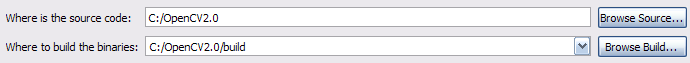
\includegraphics[scale=0.75]{images/cmake.png} 
\item Click Configure, use the VS2008 C++ compiler\\
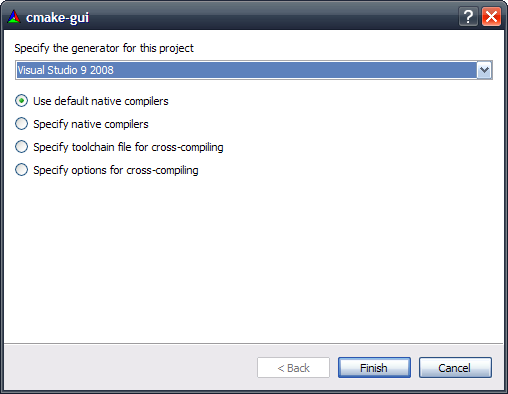
\includegraphics[scale=0.75]{images/cmake_compiler.png} 
\item In the build options make sure OpenMP is selected\\
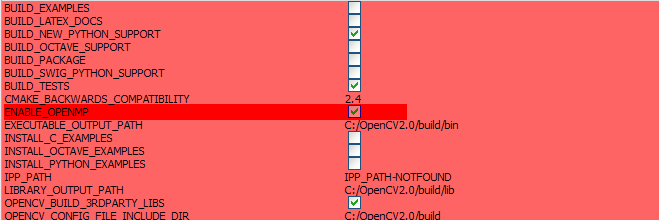
\includegraphics[scale=0.75]{images/cmake_openmp.png} 
\item Click Configure again, and then Build
\item Under \texttt{C:\textbackslash OpenCV2.0\textbackslash build} open \texttt{OpenCV.sln} 
\item Build the solution in Visual Studio under the Debug target and the Release target
\item In Visual Studio, under Tools $\rightarrow$ Options $\rightarrow$ Projects and Solutions $\rightarrow$ VC++ Directories, add the OpenCV library directories and the OpenCV include directory:\\
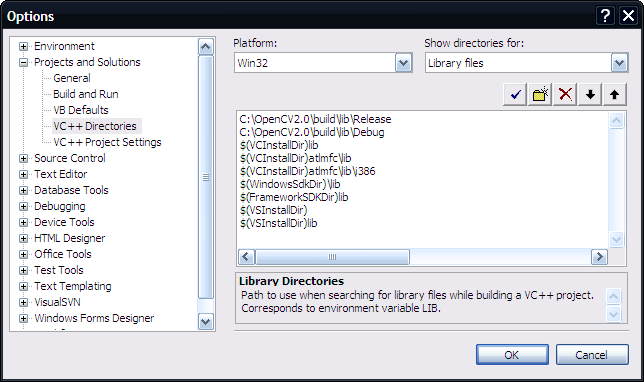
\includegraphics[scale=0.75]{images/opencv_vs.png}  \vspace*{1cm}\\
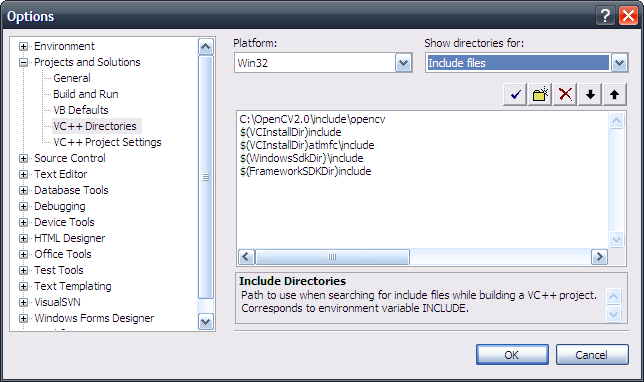
\includegraphics[scale=0.75]{images/opencv_vs_i.png} 
\item Add the following line to the system PATH environment variable: \\ \texttt{C:\textbackslash OpenCV2.0\textbackslash build\textbackslash bin\textbackslash Debug;C:\textbackslash OpenCV2.0\textbackslash build\textbackslash bin\textbackslash Release;} \\(In Computer $\rightarrow$ Properties $\rightarrow$ Advanced $\rightarrow$ Environment Variables)
\end{enumerate}

\subsection*{libconfig}
\begin{enumerate}
\item Download libconfig 1.4.6 from \\ \url{http://www.hyperrealm.com/libconfig/}
\item Extract it to \texttt{C:\textbackslash libconfig-1.4.6}
\item Open \texttt{C:\textbackslash libconfig-1.4.6\textbackslash libconfig.sln} and build the solution under the Debug and Release target.
\item Add the following line to the system PATH environment variable: \\ \texttt{C:\textbackslash libconfig-1.4.6\textbackslash Debug;C:\textbackslash libconfig-1.4.6\textbackslash Release;} \\(In Computer $\rightarrow$ Properties $\rightarrow$ Advanced $\rightarrow$ Environment Variables) 
\end{enumerate}
\subsection*{cvBlobsLib}
\begin{enumerate}
\item Download cvBlobsLib from \\ \url{http://opencv.willowgarage.com/wiki/cvBlobsLib}
\item Extract it to \texttt{C:\textbackslash cvblobslib}
\item Open \texttt{C:\textbackslash cvblobslib\textbackslash cvblobslib.dsp} and convert to a VS 2008 Solution
\item Build the solution under the Debug and Release target
\end{enumerate}
\subsection*{dlib}
\begin{enumerate}
\item Download dlib C++ from \\ \url{http://dlib.net}
\item Extract the entire archive to \texttt{C:\textbackslash dlib-17.34}
\end{enumerate}
\subsection*{PS3 Eye}
\begin{enumerate}
\item Download the CL Eye Platform Driver and the CL Eye Platform SDK from \\ \url{http://codelaboratories.com/downloads}
\item Install the driver and the SDK
\item Add the CL Eye SDK library directory to the system PATH environment variable: \\ \texttt{C:\textbackslash Program Files\textbackslash Code Laboratories\textbackslash CL-Eye Platform SDK\textbackslash Bin;} (In Computer $\rightarrow$ Properties $\rightarrow$ Advanced $\rightarrow$ Environment Variables) 
\end{enumerate}
\subsection*{Qt 4.7.1}
These installation instructions were taken from \\ \url{https://dcsoft.wordpress.com/2010/01/30/}
\begin{enumerate}
\item Download Qt from \\ \url{http://get.qt.nokia.com/qt/source/qt-everywhere-opensource-src-4.7.1.zip}
\item Extract the archive to \texttt{c:\textbackslash qt\textbackslash 4.6.1-vc}
\item Add the environment variable QTDIR: \texttt{QTDIR=c:\textbackslash qt\textbackslash 4.6.1-vc} and the following line to the system PATH environment variable: \texttt{\%QTDIR\%\textbackslash bin} (In Computer $\rightarrow$ Properties $\rightarrow$ Advanced $\rightarrow$ Environment Variables) 
\item Open a Visual Studio Command Prompt and navigate to the \texttt{c:\textbackslash qt\textbackslash 4.6.1-vc} directory
\item Type \texttt{configure -platform win32-msvc2008 } and follow the instructions
\item Type \texttt{nmake} to build Qt.
\item Make sure the following line is added to the system PATH environment variable: \texttt{c:\textbackslash qt\textbackslash 4.6.1-vc\textbackslash bin} (In Computer $\rightarrow$ Properties $\rightarrow$ Advanced $\rightarrow$ Environment Variables) 
\item Download the Visual Studio Qt Addin from \\ \url{http://qt.nokia.com/downloads/visual-studio-add-in}
\item Install the VS Qt Addin
\item In Visual Studio under Qt $\rightarrow$ Qt Options, add the Qt version 4.7.1-vc: \\ \texttt{c:\textbackslash qt\textbackslash 4.6.1-vc}

\end{enumerate}
\subsection*{EGR}
\begin{enumerate}
\item Create the \texttt{c:\textbackslash egr} directory
\item Copy the the files \texttt{tracker.cfg} and \texttt{3gest.egrdf} to this directory
\end{enumerate}
\clearpage

\section*{Train a new posture}
\begin{enumerate}
\item Record a video with \texttt{recorder.exe} (in \texttt{EGR\textbackslash Release})\\
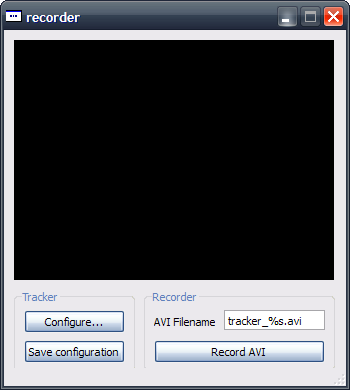
\includegraphics[scale=0.75]{images/recorder} 
\item Edit the posture labels with a subtitle editor (i.e. Subtitle Workshop from \url{http://www.urusoft.net}):
As soon the posture is visible as it is intended to be captured, set the beginning of a new subtitle label. Set the end of the subtitle label when the posture is not anymore in the intended arrangement.
\item Save the posture subtitle file in SubRip (*.srt) format, with the exact same name as the video file.
\item Launch \texttt{trainer.exe} (in \texttt{EGR\textbackslash Release}) \\
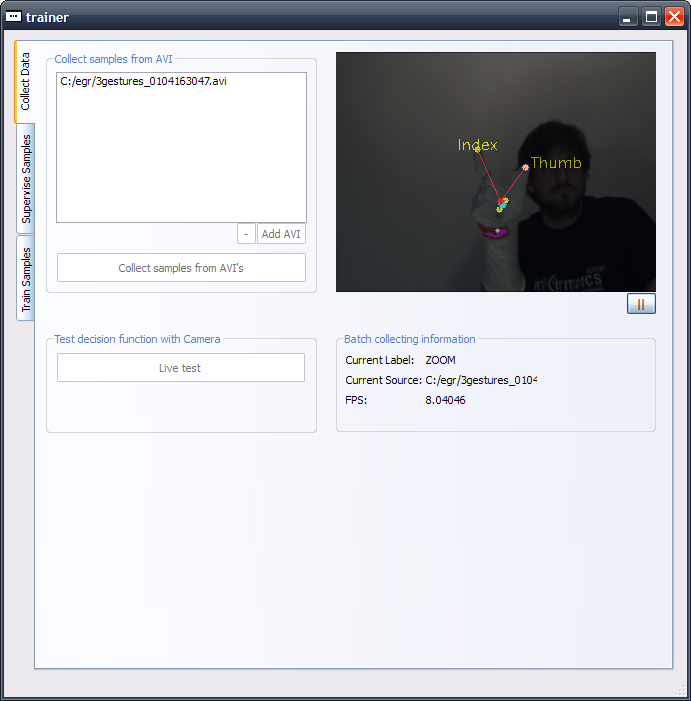
\includegraphics[scale=0.75]{images/collect-samples} 
\item Add the Video file and click \textit{Collect Samples from AVI's}
\item When the sample collection is finished, go to the \textit{Supervise samples} tab and save the samples library.\\
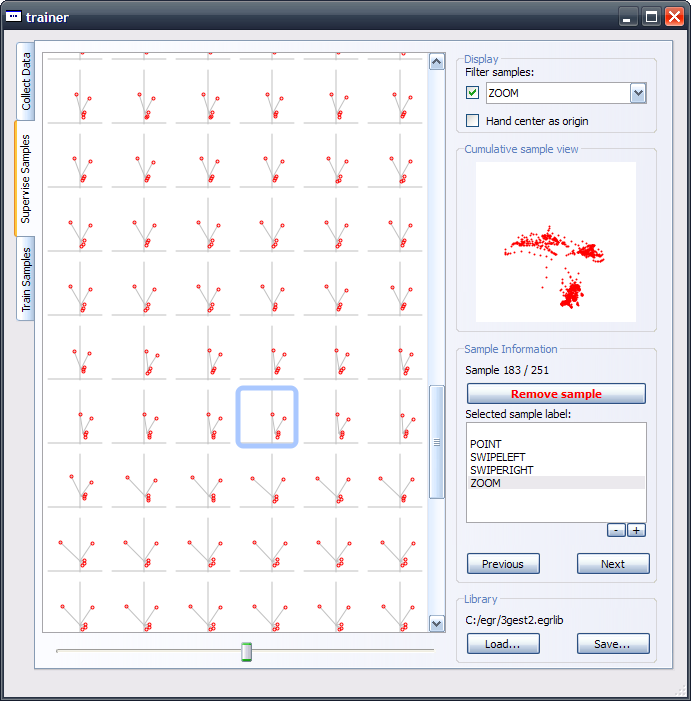
\includegraphics[scale=0.75]{images/sample-supervision} 
\item Make sure one label class contains all and only correct postures: 
\begin{itemize}
\item erase postures with coordinates far off the usual area
\item navigate with a click on the posture representation or with \textit{Previous} and \textit{Next}
\item change the label of a posture sample by clicking on the correct label in the list \textit{Selected sample label}
\end{itemize}
\item Save the supervised sample library again and go to the \textit{Train Samples} tab\\
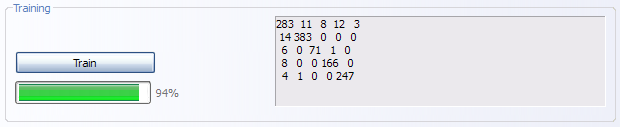
\includegraphics[scale=0.75]{images/train} 
\item Click Train. When the training is finished the progress bar indicates the accuracy in a cross-validation and the text area contains the confusion matrix of the trained decision function
\item Save the decision function
\end{enumerate}
\clearpage

\section*{Create new tracker filter}
\begin{enumerate}
\item Create a new C++ class for \texttt{NewFilter} (\texttt{NewFilter.cpp} and \texttt{NewFilter.h}) in the tracker project.
\item \texttt{NewFilter.h}:\\
\begin{lstlisting}
#pragma once
#include "filter.h"
#include "global.h"

class NewFilter :
	public Filter
{
public:
	NewFilter(void);
	~NewFilter(void);
	NewFilter* clone();
	IplImage* filter(std::vector<IplImage* > images);
}
\end{lstlisting}
\item \texttt{NewFilter.cpp}:\\
\begin{lstlisting}
#include "stdafx.h"
#include "NewFilter.h"

NewFilter::NewFilter(void)
{
	name = "New Filter"; //this name is displayed in the overlay
	sourceCount=1; //number of input images to the filter
    params.push_back(new Parameter(0.0f, 1.0f, 5.0f)); //specify range (minimum, lower bound, upper bound, maximum) with 4 float parameters
}

NewFilter::~NewFilter(void)
{
}

NewFilter* NewFilter::clone(){
	NewFilter *nf = new NewFilter();
    nf->params.clear();
    for(int i=0;i<(int)params.size();i++)
        nf->params.push_back(new Parameter(this->params[i]));
    return nf;
}

IplImage* NewFilter::filter(std::vector<IplImage*> images){
	IplImage *img = 0;
	if(images.size()>0)
		img = images[0];

	Parameter *p = params[0];
	float value = p->getVal();
	if(p != 0 ){
		//do something
	}
	return img;

}
\end{lstlisting}
\item Add the Filter to the \texttt{initFilters()} method in \texttt{main.cpp}. Make sure the name of the filter and the filter object have the same index in the \texttt{strFilterList} and the \texttt{filterList} vectors!
\begin{lstlisting}
void initFilters(){
	strFilterList.push_back("New Filter");
	strFilterList.push_back("Empty Filter");
	strFilterList.push_back("Lab Threshold Filter");
	strFilterList.push_back("Erosion Filter");
	strFilterList.push_back("Dilation Filter");
	strFilterList.push_back("Blob Filter");
	strFilterList.push_back("Add Filter");
	strFilterList.push_back("Threshold Filter");
	strFilterList.push_back("RGB Threshold Filter");
	strFilterList.push_back("Split Filter");
	strFilterList.push_back("Fast Corner Filter");
	strFilterList.push_back("Smooth Filter");
		
	filterList.push_back(new NewFilter());
	filterList.push_back(new EmptyFilter());
	filterList.push_back(new LabThresholdFilter());
	filterList.push_back(new ErosionFilter());
	filterList.push_back(new DilationFilter());
	filterList.push_back(new BlobFilter());
	filterList.push_back(new AddFilter());
	filterList.push_back(new ThresholdFilter());
	filterList.push_back(new RGBThresholdFilter());
	filterList.push_back(new SplitFilter());
	filterList.push_back(new FastCornerFilter());
	filterList.push_back(new SmoothFilter());
	
	
}
\end{lstlisting}
\item Include the new filter header file in \texttt{tracker.h}
\begin{lstlisting}
...
#include "NewFilter.h"
#include "EmptyFilter.h"
...
\end{lstlisting}
\end{enumerate}
\clearpage

\section*{Write application with EGRHand}
\begin{enumerate}
\item In Visual Studio, create a new Project within the EGR solution
\item Under Project Properties $\rightarrow$ Configuration Properties $\rightarrow$ C/C++ $\rightarrow$ General, add the following Include directories:
\begin{itemize}
\item \verb+$(SolutionDir)\model+
\item \verb+$(SolutionDir)\trainer+
\item \verb+c:\dlib-17.34+
\end{itemize}
\item Under Project Properties $\rightarrow$ Configuration Properties $\rightarrow$ Linker $\rightarrow$ General, add the following Library directory: 
\verb+$(OutDir)+
\item Under Project Properties $\rightarrow$ Configuration Properties $\rightarrow$ Linker $\rightarrow$ Input, add the following library dependecies: 
\begin{lstlisting}
model.lib
cv200.lib
highgui200.lib
cvaux200.lib
cxcore200.lib
cxts200.lib
ml200.lib
opencv_ffmpeg200.lib
\end{lstlisting}
\item Include the following header files:
\begin{lstlisting}
#include "EGRHand.h"
#include "egr_dlib.h"
#include "dlib/svm.h"
#include <iostream>
\end{lstlisting}
\item The EGRHand object is initialized as follows:
\begin{lstlisting}
EGRHand *hand = createEGRHand();
//blobs_5: the finger blobs are detected in step 5
//blobs_6: the wrist blob is detected in step 6
hand->init("c:\\egr\\tracker.cfg", "blobs_5", "blobs_6");
//load the decision function 
ifstream fin("c:\\egr\\3gest.egrdf", ios::binary);
deserialize(df, fin);
hand->setClassifier(df);
hand->start();
\end{lstlisting}
\clearpage
\item Retreive information from the EGRHand object as follows:
\begin{lstlisting}
IplImage *tracker_frame = (IplImage *) hand->getTrackerImage("Screen 8");
string posture = hand->getClassifiedPosture();
\end{lstlisting}
\item Take a look at the methods \texttt{handleGesture(string)} and \texttt{filterPostures(string, int)} in the mouse project of the EGR solution.
\end{enumerate}